\FloatBarrier
\begin{figure}
    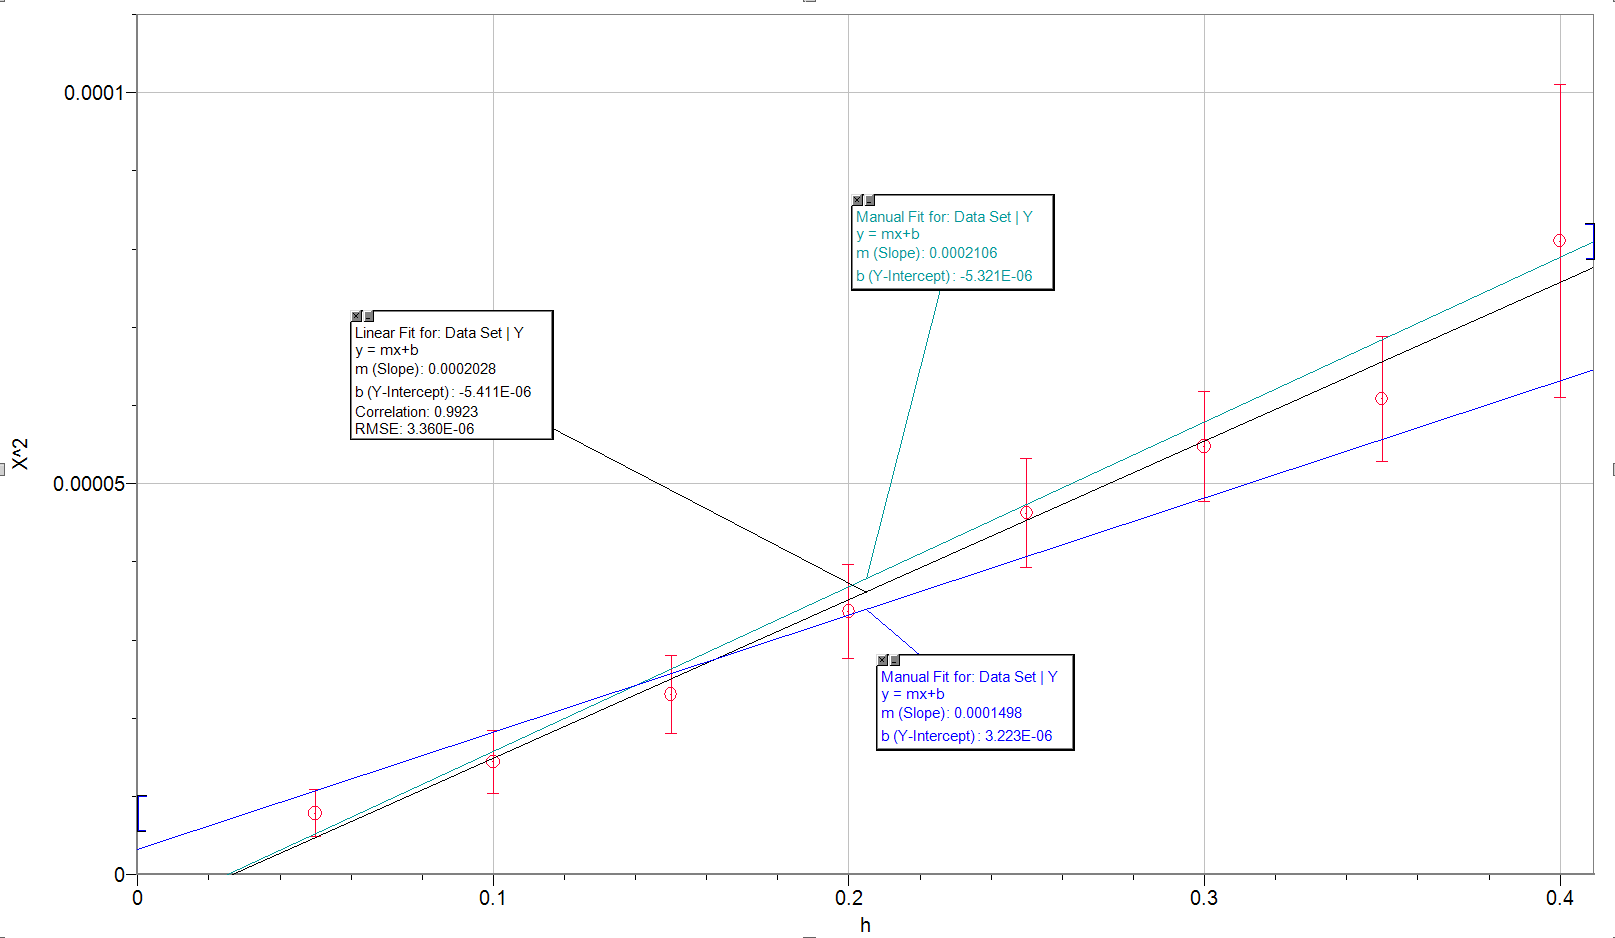
\includegraphics[width = \textwidth]{graph.png}
    \caption{Graph of $x^2$ vs $h$}
\end{figure} %make it bigger fonts
\FloatBarrier
From the graph, there is a positive correlation between $x^2$ and $h$. The best fit line has an equation of $y = 0.0002028x - 0.000005411$. Compared to the directly proportional relationship as expected, there is a small systematic error. This is probably caused by the fact that the marble drop height is measured from the surface of the table, while the spring lies on the track itself, not the table surface, so there is a small difference in height. There is no significant anomaly in the data